\documentclass[12pt]{article}
\usepackage[margin=1in]{geometry}
\usepackage{bm}
\usepackage{hyperref}
\usepackage{graphicx}
\usepackage{caption}
\usepackage{amsmath, amssymb}
\usepackage{appendix}
\usepackage{braket}
\newtheorem{theorem}{Theorem}

\usepackage{sectsty,xcolor}
\definecolor{my_color}{rgb}{0.06, 0.3, 0.57}

\title{\color{my_color}An\\ Introduction to\\ Quaternions and Rotation}
\author{Rishav}
\date{December 2020}

\begin{document}

\newpage
\maketitle
\thispagestyle{empty}

\newpage
\thispagestyle{empty}
\begin{center}
    \Large{Dedicated \\ to \\ Olinde Rodrigues}
\end{center}
~\vfill
\begin{figure}[hbt!]
\begin{center}
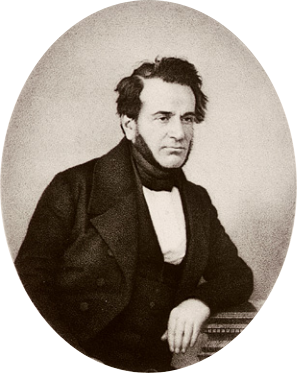
\includegraphics[width = 8cm]{figs/fig_olinde_rodrigues.png}
\caption*{Benjamin Olinde Rodrigues\\ (6 October 1795 – 17 December 1851)}
\end{center}
\end{figure}
\vfill

\newpage
\pagenumbering{arabic}
\tableofcontents

\newpage
~\vfill
\begin{figure}[hbt!]
    \begin{center}
        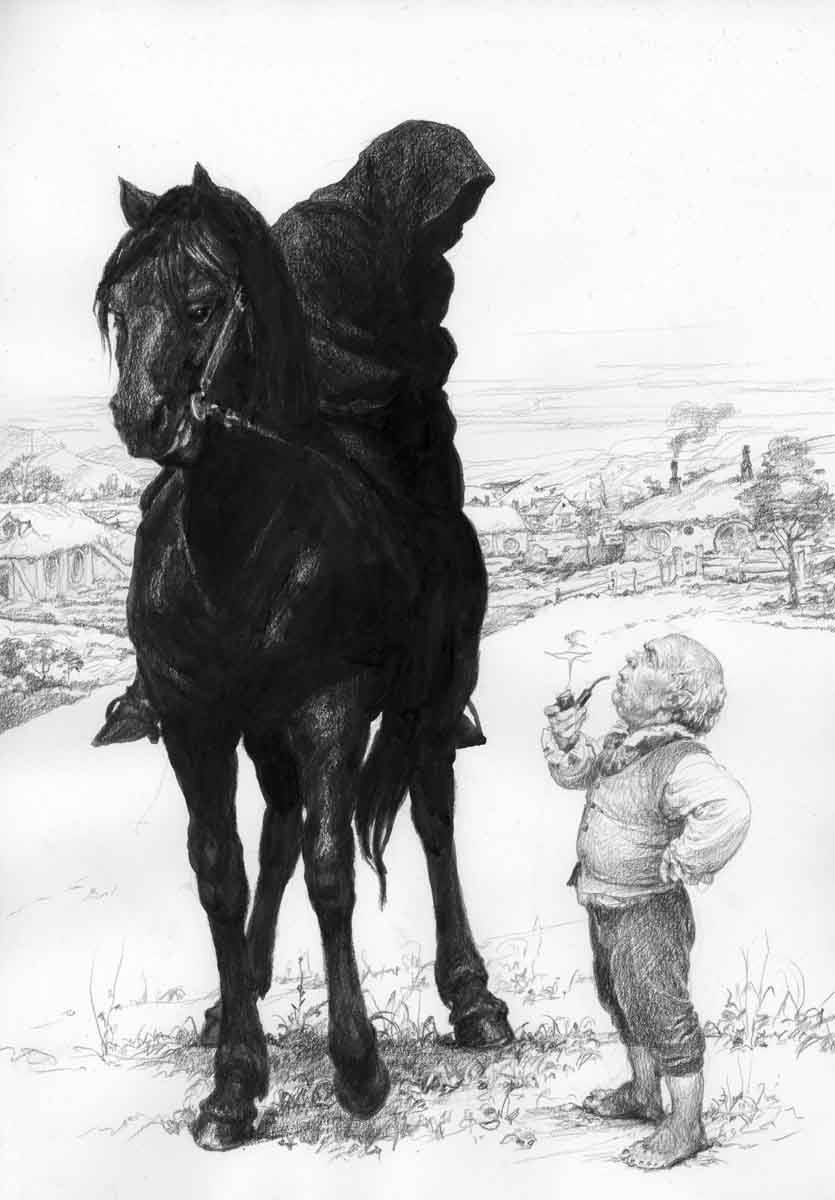
\includegraphics[width = 10cm]{figs/fig_denis_gordeev.jpg}
        \caption*{Nazgûl and a Hobbit by Denis Gordeev\\ depicts my first encounter with quaternions.}
    \end{center}
\end{figure}
\vfill

\newpage
\section{History}
The existence of complex number system and its interpretation as a point in two dimensional complex plane (plane $\mathbb{R}^{2}$ where elements belong to $\mathbb{C}$) had inspired the mathematicians to look for its three-dimensional equivalent. Moreover, the imaginary unit $\bm{i}$ being able to rotate any complex number by $90^\circ$ also had set some expectations for this three-dimensional equivalent to be interesting for its rotational characteristics. 

The generalization of the complex number, now known as quaternion, provided mathematicians with two inspirations for them to discover it:

\begin{enumerate} \itemsep0em
    \item Algebraic - Development of new number system as an algebraic structure.
    \item Geometrical - Complex mathematical object with interesting rotational properties.
\end{enumerate}

William Rowan Hamilton discovered quaternions in 1843 by following the algebraic route and he, having known the geometric potential of the quaternions, began investigating them.
However, unknown to Hamilton, Benjamin Olinde Rodrigues had already published a paper exploring some rotational properties which would apply to the quaternions. Hamilton's discovery of quaternion is well documented and interesting at the same time. He had been pondering on the problem for the algebraic generalization of the complex number. He had the feeling that the set of triplets in the form $a + bi + cj$ where, $i^{2} = j^{2} = -1$ and $a, b, c \in \mathbb{R}$, was the candidate for his new algebra. This object would be closed under addition (i.e. operation on elements of a set belongs to the same set) operation, however not with the product operation. Let, $z_{1} = a_{1} + b_{1}i + c_{1}j$ and $z_{2} = a_{2} + b_{2}i + c_{2}j$.

\begin{equation}
    \begin{split}
        z_{1} + z_{2} &= (a_{1}+a_{1}) + (b_{1} + b_{2})i + (c_{1} + c_{2})j \\
        z_{1} * z_{2} &= a_1a_2-b_1b_2-c_1c_2 + (a_1b_2 - b_1a_2)i + (a_1c_2 + 
        c_1a_2)j + b_1c_2ij + c_1b_2ji
    \end{split}
\end{equation}

It can be seen that the set defined above is closed under addition as it can be written in the form $a + bi + cj$. However it is clear that same does not applies to the product due to extra terms with $ij$ and $ji$. The set must be closed under multiplication for them to be manipulated under the laws of algebra, so it was very important for Hamilton to make sure that his mathematical structure follows the rule. He was so obsessed with the problem that there is popular anecdote of his often asking him if he had found a way to multiply triplets. 

It so happened that on the Monday morning, 16 October 1843, Hamilton was on his way to a meeting at the Royal Irish Acadamy with his wife. On the way he had the 'Eureka!' moment where he realized that what he needed was not two but three imaginary units. There in the way he found that the solution to his problem was not the triplets but the quadruplets $a + bi + cj + dk$ with following properties:

\begin{equation}
    i^{2} = j^{2} = k^{2} = ijk =  -1, \quad \quad ij = k, \quad \quad ji = -k
\end{equation}

Hamilton was so excited with the discovery that he carved his discovery on the stone of the bridge. The bridge is now commemorated by a stone plague on his honor.

\begin{figure}[hbt!]
    \begin{center}
    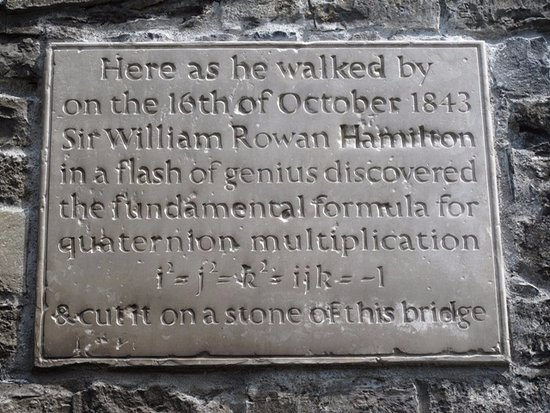
\includegraphics[width = 10cm]{figs/fig_bridge.jpg}
    \caption*{\centering \textit{Here as he walked by on the 16th of October 1843 Sir William Rowan Hamilton in a flash of genius discovered the fundamental formula for quaternion multiplication $i^{2} = j^{2} = k^{2} = ijk =  -1$ \& cut it on a stone of this bridge.}}
    \end{center}
\end{figure}

\section{Quaternion mathematics}
There are various notations to represent quaternions throughout the literature. We have adopted following notation inspired from \cite{markley2014}.

Set of all quaternions is $\mathbb{H}$ and a quaternion $\bm{q} \in \mathbb{H}$ is four dimensional vector consisting of vector part $\bm{v} \in \mathbb{R}^{3}$ and a scalar part $q_{0} \in \mathbb{R}$.

\begin{equation}
    \bm{q} = \begin{bmatrix} q_{0} \\ \bm{v} \end{bmatrix}
    \quad \quad \text{where} \quad \quad
    \bm{v} = \begin{bmatrix} q_{1} \\ q_{2} \\ q_{2} \end{bmatrix}
    \label{eqn_quat_notation}
\end{equation}

Several important mathematical characteristics of quaternion are discussed below:

\subsection{Basic operations}
Addition, subtraction and scalar multiplication can be expressed as,

$$\bm{a} = [\, a_{0} ,\: \bm{v}_{a} \,]^{\intercal} \quad \quad \bm{b} = [\, b_{0} ,\: \bm{v}_{b} \,]^{\intercal}, \quad \bm{a}, \bm{b} \in \mathbb{H}, \quad \text{and} \quad \lambda \in \mathbb{R} $$

\begin{equation}
    \begin{split}
    \text{Addition : } \bm{a} + \bm{b} &= [\, a_{0} + b_{0} ,\: \bm{v}_{a} + \bm{v}_{b} \,]^{\intercal} \\
    \text{Subtraction : }  \bm{a} - \bm{b} &= [\, a_{0} - b_{0} ,\: \bm{v}_{a} - \bm{v}_{b} \,]^{\intercal} \\
    \text{Scalar multiplication : }  \lambda \, \bm{a} &= [\, \lambda \, a_{0} ,\: \lambda \, \bm{v}_{a} \,]^{\intercal} \\
    \end{split}
\end{equation}

\subsection{Quaternion multiplication}
The product of pair of quaternions $\bm{a} = [\, a_{0} ,\: \bm{v}_{a}\,]^{\intercal}$ and $\bm{b} = [\, b_{0} ,\: \bm{v}_{b} \,]^{\intercal}$, as Hamilton defined them, is written as,

\begin{equation}
    \bm{a}\odot \bm{b} =
    \begin{bmatrix}
    a_{0} \, b_{0} -  \bm{v}_{a} \, . \, \bm{v}_{b} \\
    a_{0} \, \bm{v}_{b} + b_{0} \, \bm{v}_{a} + \bm{v}_{a} \times \bm{v}_{b} \\
    \end{bmatrix}.
    \label{eqn_hamilton_prod}
\end{equation}

\cite{markley2014} defines quaternion product with small modification to the one defined by Hamilton. This form of the quaternion product is more useful in the attitude analysis.

\begin{equation}
    \bm{a}\otimes\bm{b} =
    \begin{bmatrix}
        a_{0} \, b_{0} -  \bm{v}_{a} \, . \, \bm{v}_{b} \\
        a_{0} \, \bm{v}_{b} + b_{0} \, \bm{v}_{a} - \bm{v}_{a} \times \bm{v}_{b} \\
    \end{bmatrix}.
    \label{eqn_markley_notation}
\end{equation}

For three quaternions $\bm{a}$, $\bm{b}$ and $\bm{c}$, the quaternion multiplication follows following properties.

\begin{equation}
    \begin{split}
        \text{Associative :} \quad \bm{a} \odot (\bm{b} \odot \bm{c}) &= (\bm{a} \odot \bm{b}) \odot \bm{c} \\
        \text{Distributive :} \quad \bm{a} \odot (\bm{b} + \bm{c}) &= \bm{a} \odot \bm{b} + \bm{a} \odot \bm{c} \\
        \text{Non-commutative :} \quad \bm{a} \odot \bm{b} &\neq \bm{a} \odot \bm{b} \\
    \end{split} 
\end{equation} 

It is to be noted that the quaternions are generally non-commutative, so for special cases $\bm{a} \otimes \bm{b} = \bm{b} \otimes \bm{a}$ may exist. This can be understood analogous to the matrix multiplication. The above properties are same for $\otimes$ operation. 

\subsection{Conjugate and inverse of a quaternion}
The conjugate of a quaternion shares its origin to the conjugate of a complex number. For any complex number $\bm{z} = a + bi$, its conjugate is $\bm{z}^{*} = a - bi$ which is used to compute inverse of a complex number. Similarly for given quaternion $\bm{q} = [\, q_{0} \quad \bm{v} \,]^{\intercal}$, its conjugate is

\begin{equation}
    \bm{q}^{*} = [\, q_{0} ,\: -\bm{v} \,]^{\intercal}.
\end{equation}

Inverse of a quaternion with non zero norm is defined using its conjugate

\begin{equation}
    \bm{q}^{-1} = \frac{\bm{q}^{*}}{|\bm{q}|^{2}}
\end{equation}
where, $|\bm{q}|$ is the norm of $\bm{q}$.

\subsection{Norm of a quaternion}
Norm of a quaternion $\bm{q} = [s,\; \bm{v}]$ is defined as

\begin{equation}
    |q| = \sqrt{s^{2} + v^{2}}
\end{equation}

where, $v = |\bm{v}|$. Norm is also defined in terms of conjugate of $\bm{q}$,

\begin{equation}
    |\bm{q}| = \bm{q} \odot \bm{q}^{*}
\end{equation} 

\section{Quaternions and rotation}
In 1775, long before the discovery of quaternions by Hamilton, Leonard Euler proved that in three-dimension every rotation can be expressed as rotation about a single axis \cite{altmann1989}. The theorem is stated as follows \cite{kenechi2020}:

\begin{theorem}
    An arbitrary rotation $\bm{Q}$ in 3D is a rotation around some axis $\bm{v}$ by some angle $\psi$. 
\end{theorem}

$\bm{Q} \, \bm{v} = \bm{v}$ implies that the vector is not affected by the transformation due to rotation matrix $\bm{Q}$. The successive rotations about distinct coordinate axes is equivalent to rotation about a single axis $\bm{v}$. It was not Euler who provided the solution to find the axis $\bm{v}$. It was done by Rodrigues on 1840. This discovery of Rodrigues and how it enables quaternions to parameterize three-dimensional rotation is is discussed in the next section.  

\subsection{Axis-angle representation of quaternions}
Let $\bm{Q}(\psi \bm{v})$ represent the rotation around axis $\bm{v} \in \mathbb{R}^{3} $ by angle $\psi$. Using this notation, following product is considered.

\begin{equation}
    \bm{Q}(\alpha \bm{l}) \, \bm{Q}(\beta \bm{m}) = \bm{Q}(\gamma \bm{n})
    \label{eqn_rodrigues_rot}
\end{equation}

Here, rotation around $\bm{m}$ by $\beta$ is followed by rotation around $\bm{l}$ by $\alpha$. Using the geometrical construction employing spherical triangle, Rodrigues found the expression for resultant axis $\bm{n}$ and the angle of rotation $\gamma$.  

\begin{equation}
    \begin{split}
        \text{cos}\frac{\gamma}{2} &= \text{cos}\frac{\alpha}{2} \, \text{cos}\frac{\beta}{2} - \text{sin}\frac{\alpha}{2} \, \text{sin}\frac{\beta}{2} \\
        \text{sin}\frac{\gamma}{2} \, \bm{n} &= \text{sin}\frac{\alpha}{2} \, \text{cos}\frac{\beta}{2} \, \bm{l} + \text{cos}\frac{\alpha}{2} \, \text{sin}\frac{\beta}{2} \, \bm{m} + \text{sin}\frac{\alpha}{2} \, \text{sin}\frac{\beta}{2} \, (\bm{l} \times \bm{m}) \\
    \end{split}
\label{eqn_rodrigues}
\end{equation}

This was the first time when the concept of half angle was introduced to the study of rotations. This opened a new way to interpret rotations, because the rotation $\bm{Q}(\gamma \bm{n})$ could now be parameterized using a scalar $cos(\gamma/2)$ and a vector $sin(\gamma/2) \, \bm{n}$. This way of representation of rotation as axis-angle representation.

The interesting feature of the Eqn.\,(\ref{eqn_rodrigues}) is that it represents the quaternion multiplication of Eqn.\,(\ref{eqn_hamilton_prod}). We can use this connection to develop new notation and interpretation of quaternions. Let us rewrite $\bm{Q}(\psi \bm{v})$ in quaternion notation of Eqn.\,(\ref{eqn_quat_notation}).

\begin{equation}
    \bm{Q}(\psi \bm{v}) \equiv \bm{q} =
    \left[\,\text{cos} \frac{\psi}{2} ,\: \text{sin} \frac{\psi}{2} \, \bm{v}^{\intercal}\, \right]
\end{equation}

Following this notation and the fact that Eqn.\,(\ref{eqn_rodrigues}) is equivalent to the quaternion multiplication we can write the resultant rotation $\bm{Q}(\gamma \bm{n})$ in Eq\,(\ref{eqn_rodrigues_rot}) as follows,

\begin{equation}
    \begin{split}
        \bm{Q}(\gamma \bm{n}) &\equiv
        \left[\,\text{cos} \frac{\gamma}{2} ,\:\text{sin} \frac{\gamma}{2} \, \bm{n}^{\intercal}\, \right] \\   
        &=
        \left[\,\text{cos} \frac{\alpha}{2} ,\: \text{sin} \frac{\alpha}{2} \, \bm{l}^{\intercal}\, \right]
        \odot
        \left[\,\text{cos} \frac{\beta}{2} ,\: \text{sin} \frac{\beta}{2} \, \bm{m}^{\intercal}\, \right]
    \end{split} 
\end{equation}

This suggests that the Hamilton multiplication of two quaternions corresponds to the successive rotations about the different axes represented by each of them.

The implications of the axis-angle representation of quaternions can be summarized as follows:

\begin{enumerate}
    \item Arbitrary unit quaternion $\bm{q}$ can be interpreted as the mathematical object that represents a three-dimensional rotation by an angle of $\psi$ about an axis $\bm{v} \in \mathbb{R}^{3}$.
    $$\bm{q} = \left[\, \text{cos}\frac{\psi}{2} ,\: \text{sin}\frac{\psi}{2} \, \bm{v}^{\intercal}  \, \right]^{\intercal}$$
    \item Rotation resulting from two successive rotations $\bm{q}_{1}$ and $\bm{q}_{2}$ $(\bm{q}_{1}, \bm{q}_{2} \in \mathbb{H})$ is represented by their product $\bm{q}$.
    $$\bm{q} = \bm{q}_{2} \odot \bm{q}_{1}$$ 
\end{enumerate}

In the next section, unit quaternion $\bm{q} = [cos(\psi/2), \; \bm{v} \, sin(\psi/2)]$ is recognized as the operator to rotate any three dimensional real vector about the axis $\bm{v}$ by an angle $\psi$.  

\subsection{Quaternion as rotation operator}
Orthogonal matrix $\bm{Q} \in \mathbb{R}^{3\times3}$ parameterizes rotation like quaternion does. $\bm{Q}$ can rotate $\bm{v} \in \mathbb{R}^{3}$, by vector-matix multiplication.

\begin{equation}
    \bm{v}' = \bm{Q} \, \bm{v}
\end{equation}

Where, $\bm{v}'$ is the new vector after the rotation of $\bm{v}$. Quaternions can also operate on vector to produce resulting rotated vector like the rotation matrices do. 

There is an important algebraic considerations to be made before dealing with this property of quaternions. Since we are looking for quaternion operation to rotate vector, one can question on how a quaternion, which lives in $\mathbb{R}^{4}$, operate on a vector, which lives in $\mathbb{R}^{3}$. The answer to this lies on the fact that vector $\bm{v} \in \mathbb{R}^{3}$ can simply be treated as though it were a quaternion $q \in \mathbb{R}^{4}$ whose real part is zero (pure quaternion). We can formally allow the existence of above quaternion-vector operation because consistent one-to-one correspondance between sets $\mathbb{R}^{3}$ and $\mathbb{H}_{0}$ (set of pure quaternions) can be established, that is
\begin{equation}
\bm{v} \in \mathbb{R}^{3} \leftrightarrow \bm{q} \in \mathbb{H}_{0} \subset \mathbb{H}
\end{equation}
 
Let $\bm{a} \in \mathbb{R}^{3}$ be any vector that we wish to rotate using $\bm{q} \in \mathbb{H}$ to produce $\bm{b} \in \mathbb{R}^{3}$. This operation can be expressed as,
\begin{equation}
\bm{b} = \bm{q}\,\bm{a}\,\bm{q}^{*}
\end{equation}

where, $\bm{q}^{*}$ is the conjugate of $\bm{q}$. Sandwiching vector between quaternion and its conjugate does the same operation as the multiplication by of rotation matrix equivalent to $\bm{q}$. 

\subsection{Quaternion to rotation matrix}
Let $\bm{q} = [\, q_{0}, \: q_{1}, \: q_{2}, \: q_{3} \,]^{\intercal} = [\, q_{0}, \: \bm{v}^{\intercal} \,]^{\intercal}$ be unit quaternion and $\bm{Q} \in \mathbb{R}^{3}$ be the orthogonal rotation matrix representating same rotation as that of $\bm{q}$. $\bm{Q}$ can be expressed in terms of the elements of $\bm{q}$,

\begin{equation}
    \bm{Q}(\bm{q}) = 
    \begin{bmatrix}
        q_{0}^{2}+q_{1}^{2}-q_{2}^{2}-q_{3}^{2} && 2(q_{1}q_{2}+q_{0}q_{3}) && 2(q_{1}q_{3}-q_{0}q_{2}) \\
        2(q_{1}q_{2}-q_{3}q_{2}) && q_{0}^{2}-q_{1}^{2}+q_{2}^{2}-q_{3}^{2} && 2(q_{2}q_{3}+q_{0}q_{1}) \\
        2(q_{1}q_{3}+q_{0}q_{2}) && 2(q_{2}q_{3}+q_{0}q_{1}) && q_{0}^{2}-q_{1}^{2}-q_{2}^{2}+q_{3}^{2}\\
    \end{bmatrix}
    \label{eq_quat_to_rot}
\end{equation}   

In compact form, above equation can be expressed as,
\begin{equation}
\bm{Q}(\bm{q}) = (q_{0}^{2} - |\!| \bm{v}|\!|^{2}) \bm{I} - 2q_{0}[\bm{v} \times] + 2\bm{v}\bm{v}^{\intercal}
\end{equation}

where, $[\bm{v} \times]$ is skew symmetric cross product matrix.
$$
[\bm{v} \times] \equiv 
\begin{bmatrix} 
    0 & -v_{3} & v_{2} \\ v_{3} & 0 & -v_{1} \\ -v_{2} & v_{1} & 0 
\end{bmatrix} 
$$

\subsection{Double cover}
Quaternions are not unique for the three dimensional rotations. That is, two quaternion can describe same rotation. This can be realized by observation of Eqn.\,(\ref{eq_quat_to_rot}). It can be seen that all parameters of the quaternions appear as the quadratic product, so changing the sign of all parameters produces same rotation matrix. 

The axis-angle representation of quaternion provides more intuitive description of this effect. Quaternion $\bm{q} = [cos(\psi/2), \; sin(\psi/2) \, \bm{v}]'$ represents a rotation by an angle of $\psi$ about the axis $\bm{v}$. Experience on rotation of  three dimensional rigid body shows that that rotation by $\psi = 2\pi$ should produces same orientation. However, due to the presense of half angle in quaternion, the sign of all the components of quaternion are changed i.e. $\bm{q} = -\bm{q}$. This suggests that the pair of quaternions representing same rotation are negative of one another.

\

\subsection{Rotation matrix to quaternion}
Sheppard's algorithm is the most widely applied convert rotation matrix to quaternion. It is because this algorithm is singularity free (i.e. divide by zero case). The algorithm presented here is based on \cite{markley2008}.

Let $\bm{Q} \in \mathbb{R}^{3}$ be the orthogonal rotational matrix and $\bm{q} = [\, q_{0} ,\: q_{1} ,\: q_{2},\: q_{3}\,]^\intercal$ be unit quaternion. First of all, $q_{i}^{2}$ are computed using following relations,

\begin{equation}
    \begin{split}
        4q_{0}^{2} &= 1 + \text{tr}\bm{Q} \\
        4q_{1}^{2} &= 1 - \text{tr}\bm{Q} + 2\,\bm{Q}_{11} \\
        4q_{2}^{2} &= 1 - \text{tr}\bm{Q} + 2\,\bm{Q}_{22} \\
        4q_{3}q_{4} &= 1 - \text{tr}\bm{Q} + 2\,\bm{Q}_{33} \\
    \end{split}
    \label{eqn_find_large}
\end{equation}

The largest value of $q_{i}^{2}$ is from Eqn.\,(\ref{eqn_find_large}) is used as seed to compute other $q_{j}$ $(j \neq i)$ by using appropriate three equations from six of the equations below.

\begin{equation}
    \begin{split}
        4q_{0}q_{1} &= \bm{Q}_{23} - \bm{Q}_{32} \\
        4q_{0}q_{2} &= \bm{Q}_{31} - \bm{Q}_{13} \\
        4q_{0}q_{3} &= \bm{Q}_{12} - \bm{Q}_{21} \\
        4q_{2}q_{3} &= \bm{Q}_{23} - \bm{Q}_{32} \\
        4q_{3}q_{1} &= \bm{Q}_{31} - \bm{Q}_{13} \\
        4q_{1}q_{2} &= \bm{Q}_{12} - \bm{Q}_{21} \\
        \end{split}
        \label{eqn_six}
\end{equation}

Two unit quaternions can produce same rotation matix due to double cover. Each of these two quaternions can be obtained by using either positive root or negative root of $q_{i}$ respectively. Shepperd's algorithm produces precisely normalized unit quaternion only for precisely orthogonal $\bm{Q}$.

\subsection{Error Quaternion}
In context of attitude control system, the goal is to actuate the satellite such that the orientation of satellite drives from current orientation $\bm{q}$ to desired quaternion $\tilde{\bm{q}}$. This problem is equivalent to driving error quaternion $\bm{\delta q}$ to identity, where $\bm{\delta q}$ is defined as,

\begin{equation}
    \delta\bm{q} = \bm{q} \otimes \tilde{\bm{q}}^{-1} = |\!|\tilde{\bm{q}}|\!| ^{-2}\bm{q} \otimes \tilde{\bm{q}}^{*}
\end{equation}

\section{Quaternion kinematics}
Three dimensional rigid body kinematics for quaternion is the coupled differential equation which 

The three dimensional kinematics of rigid body parameterized in quaternions is represented by four coupled differential equations which can be written in matrix form \cite{hanspeter2009}.

\begin{equation}
    \begin{bmatrix} 
        \dot{q}_{0} \\ \dot{q}_{1} \\ \dot{q}_{2} \\ \dot{q}_{3}
    \end{bmatrix}
    = \frac{1}{2}
    \begin{bmatrix}
        0 & -\omega_{1} & -\omega_{2} & -\omega_{3} \\
        \omega_{1} & 0 & \omega_{3} & -\omega_{2} \\
        \omega_{3} & -\omega_{3} & 0 & \omega_{1} \\
        \omega_{3} & \omega_{2} & -\omega_{1} & 0 \\
    \end{bmatrix}
    \begin{bmatrix} 
        q_{0} \\ q_{1} \\ q_{2} \\ q_{3}
    \end{bmatrix}
    \label{eqn_quat_diff}
\end{equation}

Eqn.\,(\ref{eqn_quat_diff}) can also be written such that the matrix now has the elements of quaternion \cite{hanspeter2009}. 

\begin{equation}
\begin{bmatrix} 
\dot{q}_{0} \\ \dot{q}_{1} \\ \dot{q}_{2} \\ \dot{q}_{3}
\end{bmatrix}
= \frac{1}{2}
\begin{bmatrix}
q_{0} & -q_{1} & -q_{2} & -q_{3} \\
q_{1} & q_{0} & -q_{3} & q_{2} \\
q_{2} & q_{3} & q_{0} & -q_{1} \\
q_{3} & -q_{2} & q_{1} & q_{0} \\
\end{bmatrix}
\begin{bmatrix}
0 \\ \omega_{1} \\ \omega_{2} \\ \omega_{3}
\end{bmatrix}
\label{eqn_quat_diff_i}
\end{equation}
 
% The numerical integration of either Eqn.\,(\ref{eqn_quat_diff}) or Eqn.\,(\ref{eqn_quat_diff_i}) can be used to simulate the rotation of rigid body parameterized in quaternions. Above equations cal be written compactly as follows,

% \begin{equation}
    
% \end{equation}

\subsection{Discrete-time quaternion kinematics}
In the OBC of satellite, $\omega_{i}$'s are determined using gyro measurements. Generally, gyro sampling occurs at high rate, this makes the discrete implementation good enough to propagate the quaternion over time. Given the known values of quaternion $\bm{q}_{k}$ and angular velocity $\bm{\omega}_{k}$ in a timestep $k$, the quaternion on the next timestep $\bm{q}_{k+1}$ can be determined by equation below \cite{crassidis2011}.

\begin{equation}
    \bm{q}_{k+1} = \bar{\bm{\Omega}}(\bm{\omega}_{k}) \, \bm{q}_{k}
\end{equation}

with,

\begin{equation*}
    \bar{\bm{\Omega}} =
    \begin{bmatrix}
        \text{cos}\left( \frac{1}{2} |\!| \bm{\omega}_{k} |\!| \Delta t \right) \bm{I}_{3\times3} & - \bm{\psi}_{k} \\
        - \bm{\psi}_{k}^{\intercal} & \text{cos}\left( \frac{1}{2} |\!|\bm{\omega}_{k}|\!| \Delta t \right)
    \end{bmatrix}
\end{equation*}

where,
\begin{equation}
\bm{\psi}_{k} \equiv \frac{sin\left( \frac{1}{2} |\!| \bm{\omega}_{k} |\!| \Delta t \right)}{|\!| \bm{\omega}_{k} |\!|}
\end{equation}

This discrete-time kinematics of quaternion is implemented in the attitude estimation algorithm used in this project. For the high frequency gyro sampling, this formulation provides accurate approximation hence avoiding the numerical integration of continuous-time equations Eqn.\,(\ref{eqn_quat_diff}) and Eqn.\,(\ref{eqn_quat_diff_i}).

\section{Advantages of quaternion parameterization}
\label{subsection:quaternion_advantages}
Major characteristics of the quaternion that makes it a good choice for attitude parameterizartion for spacecraft are listed below:

\begin{enumerate}
\item It is evident that Eqn.\,(\ref{eqn_quat_diff}) and Eqn.\,(\ref{eqn_quat_diff_i}) do not contain 0/0 type mathematical singularities which is common in all three attitude parameterization Hanspeter.

\item Rotation matrix expressed in terms of quaternions only contains the quadratic product of its element. Absence of the transedance function makes them computationally efficient for digital implementations.

\item Quaternions are parameterized using four numbers and one unit norm constraints. This is lot less than the rotation matrix which requires nine parameters ans six constraints for orthogonality.  

\item Result of two successive rotations is easily obtained by quaternion multiplication.
\end{enumerate}

\newpage
\bibliographystyle{plain}
\bibliography{references}

\end{document}
